\chapter{Desarrollo del sistema}

\bigskip
En este capítulo veremos la arquitectura del sistema, la \textit{filosofía} o principios seguidos y algunas partes del sistema.

\bigskip
El código del sistema se encuentra en GitHub. Para el sistema completo, que recoge el servicio web y la gestión de la ejecución del algoritmo genético: \textcolor{blue}{\underline{\href{https://github.com/JCristobal/SWGPU}{SWGPU}}}. Y para el módulo que gestiona el algoritmo genético: \textcolor{blue}{\underline{\href{https://github.com/JCristobal/geneticAlgorithm}{geneticAlgorithm}}}.


\bigskip
\section{Arquitectura del sistema}
\bigskip

La arquitectura del sistema está compuesta por 2 capas: BackEnd y FrontEnd. La capa de BackEnd se sitúa en el servidor, mientras que la de FrontEnd en el lado del cliente.

\bigskip
La estructura básica de la web la formará desde el lado BackEnd (en el servidor) mediante Django (usando python) y será servida por el servidor Apache. 

El cliente, desde el FrontEnd, verá la web mediante HTML5, CSS3 y JavaScript, y podrá interactuar con ella fácilmente gracias a las funcionalidades de jQuery y AngularJS

Otra vez en el BackEnd, tras la petición del cliente, el algoritmo genético se ejecutará en C++ y CUDA. La respuesta se le enviará en formato JSON, para ser maquetada de forma correspondiente.


\bigskip
En la siguiente imagen (Figura \ref{fig:estructura}) se muestra con sus distintos elementos:

\bigskip
\begin{figure}[h]
	\centering
	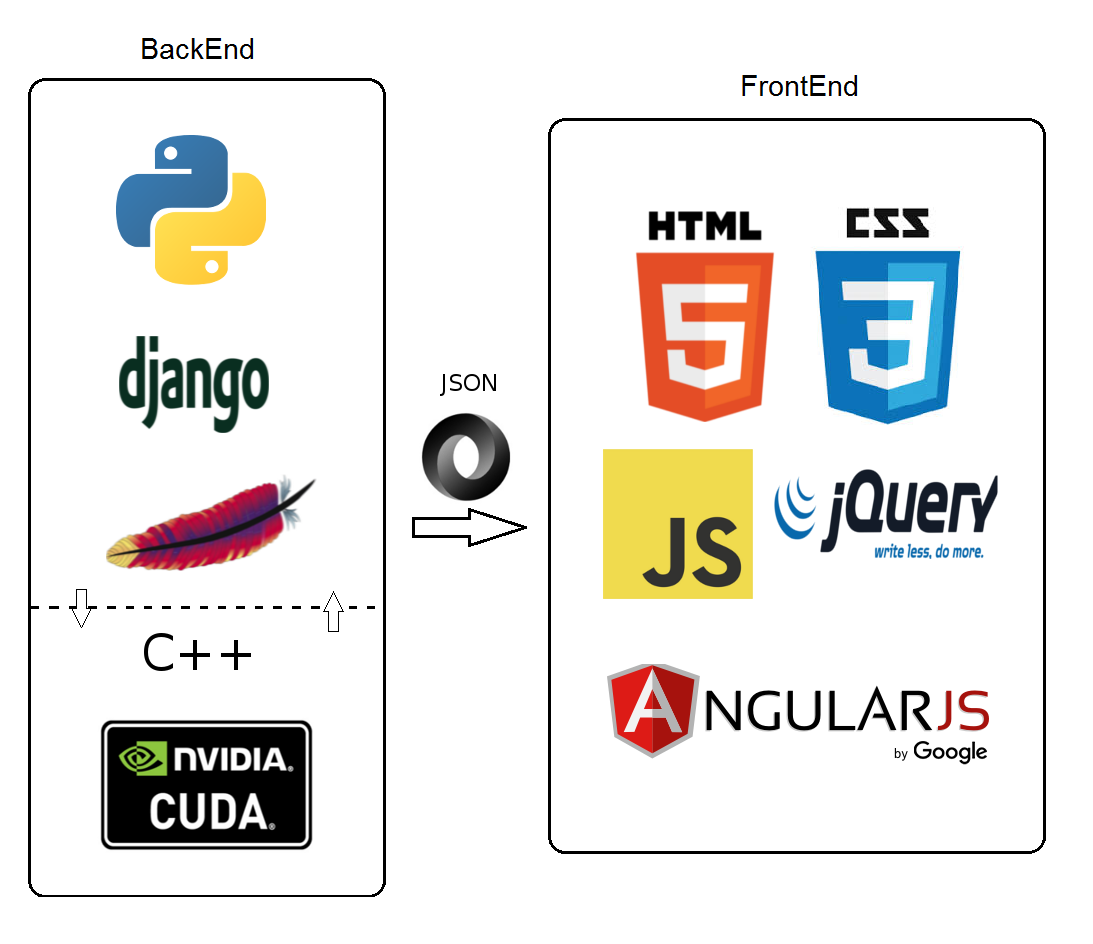
\includegraphics[width=1\linewidth]{../images/estructura}
	\caption[Estructura del sistema]{Estructura del sistema}
	\label{fig:estructura}
\end{figure}



\newpage
\section{Partes del sistema}

\bigskip
\textbf{BackEnd}\\

Será el lado del servidor de la aplicación. Basado en Django (y disponible mediante el servidor Apache), con éste tenemos acceso a los recursos del servidor, entre ellos la GPU. Con Django formaremos la petición según los parámetros que ha especificado el cliente, y se hará uso de la GPU mediante CUDA. Django tendrá la salida del cálculo, y la devolverá en un formato determinado.

Se puede decir que el BackEnd tiene 2 partes: el servidor web y el procesado dentro del servidor.

\bigskip
\textbf{FrontEnd}\\

Lado que ve el cliente, el FrontEnd. Con las tecnologías básicas web (HTML5, CSS y JavaScript) se creará una interfaz para el cliente. Mediante jQuery y AngularJS podrá interactuar fácilmente y con fluidez, además de servir la respuesta que le da el servidor.

\bigskip
AngularJS se encarga de la comunicación con el BackEnd a través de servicios, y con esos datos actualiza la interfaz. Conforma un modelo MVC (Modelo Vista Controlador), que separa los datos y su gestión (componente de modelo) de la aplicación de la interfaz de usuario (vista) y el módulo encargado de gestionar los eventos y las comunicaciones (controlador).

MVC propone la construcción de tres componentes distintos (modelo, vista y controlador): por un lado define componentes para la representación de la información, y por otro lado para la interacción del usuario. 

\bigskip
\begin{figure}[h]
	\centering
	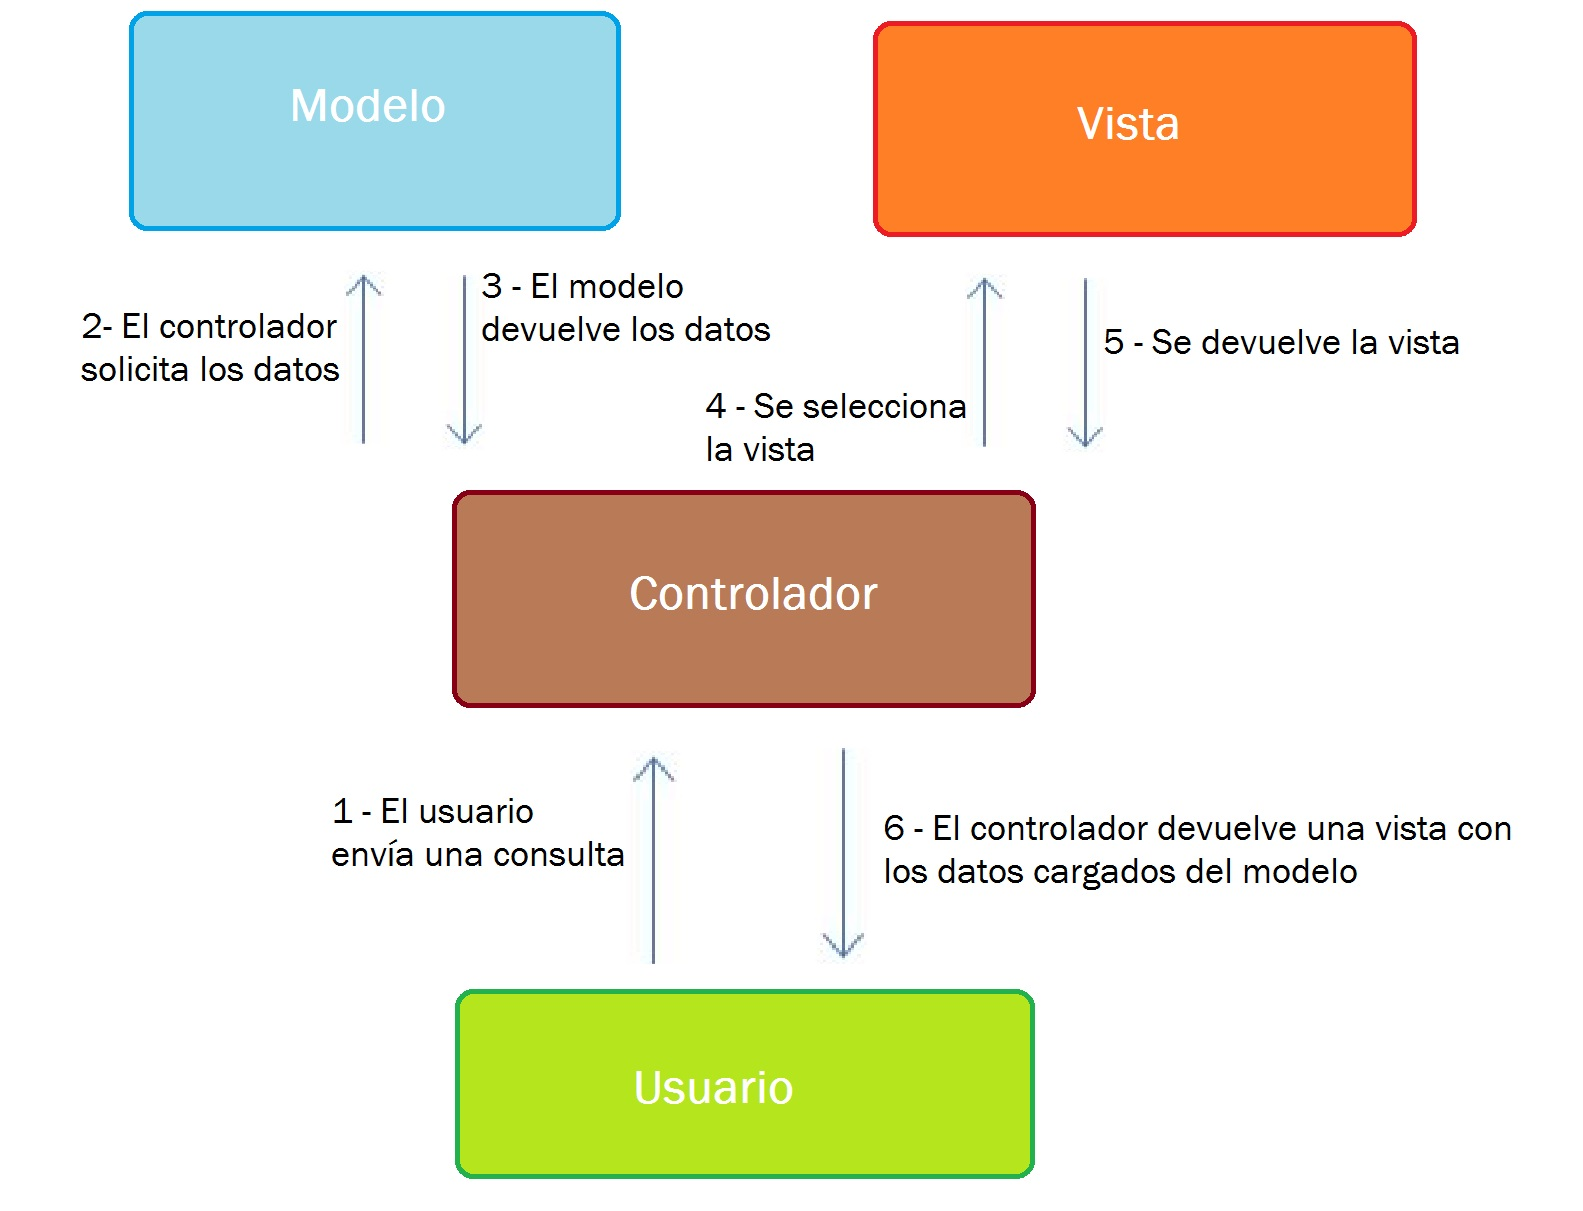
\includegraphics[width=0.8\linewidth]{../images/mvc}
	\caption[Modelo Vista Controlador]{Modelo Vista Controlador}
	\label{fig:mvc}
\end{figure}



\newpage
\section{Filosofía a seguir}
\bigskip
A la hora de implementar y de realizar el trabajo en general se ha intentado ser lo más ordenado y pulcro posible, esto en un principio  puede ralentizar el proceso, pero a largo plazo hace que el desarrollo, actualización o mantenimiento del sistema sea más rápido y fácil. Estos son algunos de los criterios empleados en el desarrollo.

\bigskip
\subsection{Desarrollo general}
\bigskip

Las funciones del sistema se han desarrollado de la manera más general posible para así favorecer la reutilización de código y facilitar su legibilidad. También son más fáciles de mantener puesto que al ser de ámbito más general son más mantenibles.

\bigskip
\subsection{Modularización}
\bigskip

Se ha desarrollado el código en distintos módulos. De esta forma se evita que al hacer cambios en un módulo se propague a los demás, lo que hace el código más mantenible y eficiente.

\bigskip
\subsection{Control de versiones}
\bigskip

Se apostó por un sistema de control de versiones, en mi caso Git mediante la plataforma GitHub \cite{github}, ya que favorece el mantenimiento de las distintas versiones de código de una manera sencilla y rápida.

El manejo de Git es sencillo, ya que con unas cuantas ordenes se puede manejar sin problemas, y GitHub está provisto de una interfaz muy intuitiva. 

\bigskip
Algunas de las órdenes que se han usado para el trabajo son:\\


\textit{git clone[URL del proyecto]}: se descarga el proyecto del repositorio Git.\\


\textit{git add [archivos]}: añade los archivos con los cambios deseados en un "paquete" para el commit.\\


\textit{git commit}: subida de los archivos especificados al repositorio local.\\


\textit{git push}: propaga los cambios locales al repositorio.\\


\textit{git pull origin}: Actualiza la versión del código.\\


\textit{git status}: muestra el estado de los archivos.\\


\bigskip
\subsection{Desarrollo iterativo incremental}
\bigskip

El desarrollo de las funcionalidades se hace de forma progresiva, de modo que primero se implementan las más críticas y prioritarias en primer lugar para poder tener siempre un producto funcional.

\bigskip
\subsection{Revisiones periódicas del código}
\bigskip

El código es revisado tras cada interacción de desarrollo, con el fin de mantenerlo lo más pulcro y estructurado posible. De este modo se evitan repeticiones en el código o dejar partes incompletas. Así se proporciona un mayor nivel de calidad a código producido.

\bigskip
\subsection{Documentación del código}
\bigskip

El código ha sido documentado, de modo que es más mantenible por terceros y por el mismo autor. Cada funcionalidad ha sido detallada debidamente, de manera clara y concisa, sin extender demasiado la explicación.




\newpage
\section{Estructura}

\bigskip
\subsection{FrontEnd}
\bigskip

Sigue el modelo que recomienda AngularJS, como antes se cita, se basa en el modelo MVC. Los distintos tipos de archivos que formarán las \textit{vistas} (en distintas ubicaciones según la forma de Django) son:

\begin{itemize}
	\item HTML (dentro del directorio \textit{templates}) será la plantilla visible del sistema.
	\item CSS: (en el directorio \textit{static/assets/css}) estilos que usará HTML.
	\item JavaScript (dentro de \textit{static/assets/js}) mediante jQuery y AngularJS permitirán interactuar con el sistema.
	\item Las imágenes y distintas librerías que se usen también se ubicarán en \textit{static/assets}.
\end{itemize}


\bigskip
\subsection{BackEnd}
\bigskip

Se hará uso de Django para crearlo y gestionarlo. A continuación se citan sus partes importantes que se usan en el proyecto:

\begin{itemize}

	\item \textbf{manage.py}: archivo para gestionar el proyecto (inspeccionarlo en busca de problemas, lanzar el servidor o cargar datos).
	\item \textbf{settings.py}: configuraciones del proyecto (dirección de algunos directorios o carga de módulos con distintas funcionalidades)
	
	Dentro del directorio \textit{swgpu} (que será un \textit{packete python}):
	\begin{itemize}
		\item \textbf{urls.py}: URL declaradas dentro del proyecto \textit{swgpu}.
		\item \textbf{views.py}: para gestionar las vistas y las funcionalidades del proyecto.
	\end{itemize}
	
	
	\item La parte de FrotEnd antes descrita se situará en los directorios \textit{templates} y \textit{static}. Django hará uso de los distintos archivos dentro para lanzar y trabajar con el servicio web.
\end{itemize}

\bigskip
\subsection{Ejecutable a usar por el BackEnd}
\bigskip

El sistema hará uso de la GPU del servidor (BackEnd) mediante el ejecutable \textit{geneticAlgorithm} (ubicado en el directorio \textit{bin}), escrito en C++ y CUDA. De esta manera se facilitará el servicio, ya que al tratarse de un ejecutable al que sólo hay que realizar una petición con los parámetros deseados se cubren los posibles fallos y la salida que dará. 

\bigskip
En las siguiente imagen se ve una captura de petición de ayuda sobre las variables a introducir mediante el ejecutable:

\bigskip
\begin{figure}[h]
	\centering
	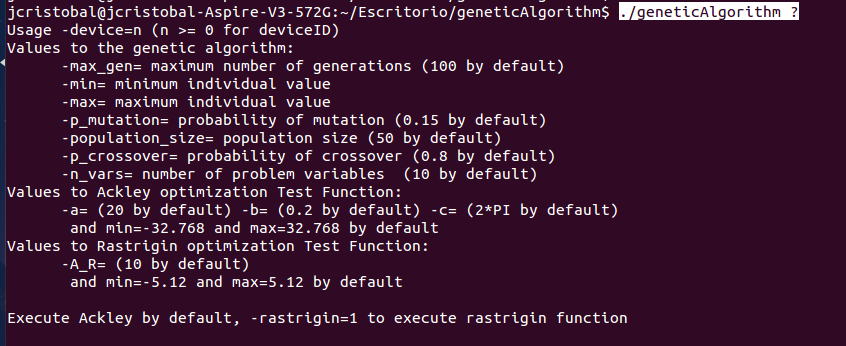
\includegraphics[width=1\linewidth]{../images/peticion_ejecutable}
	\caption[Petición de un algoritmo genético mediante el ejecutable]{Petición de un algoritmo genético mediante el ejecutable}
	\label{fig:peticion_ejecutable}
\end{figure}

\bigskip
Y otra captura con una petición que ejecutaría el algoritmo genético con los parámetros especificados además de los declarados por defecto:

\bigskip
\begin{figure}[h]
	\centering
	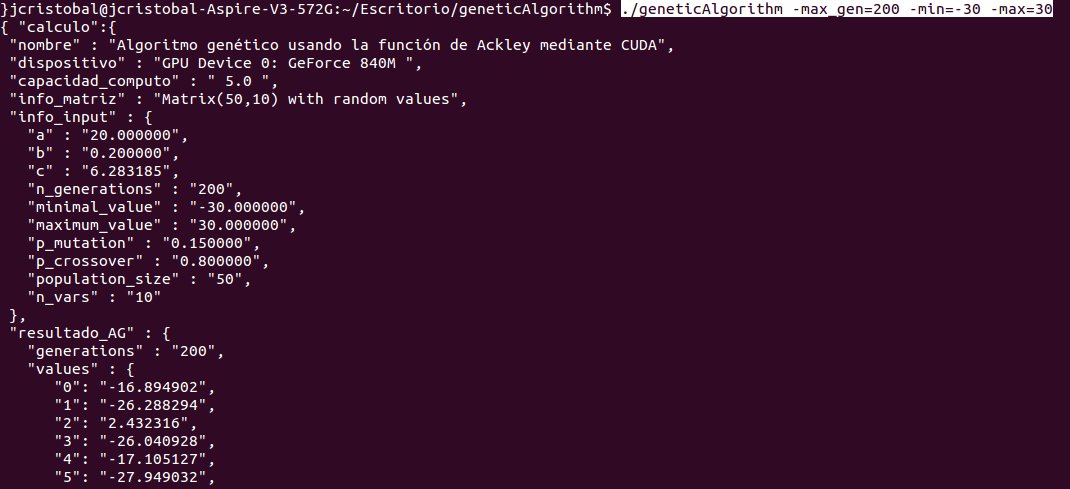
\includegraphics[width=1\linewidth]{../images/salida_ejecutable}
	\caption[Salida del algoritmo genético]{Salida del algoritmo genético}
	\label{fig:salida_ejecutable}
\end{figure}

\bigskip
y a continuación se ve la salida completa en formato JSON:

\begin{lstlisting}
{
	"calculo": {
		"nombre": "Algoritmo genético usando la función de Ackley mediante CUDA",
		"dispositivo": "GPU Device 0: GeForce 840M ",
		"capacidad_computo": " 5.0 ",
		"info_input": {
			"a": "20.000000",
			"b": "0.200000",
			"c": "6.283185",
			"n_generations": "200",
			"minimal_value": "-30.0000",
			"maximum_value": "30.0000",
			"p_mutation": "0.150000",
			"p_crossover": "0.800000",
			"population_size": "50",
			"n_vars": "10"
		},
		"resultado_AG": {
			"generations": "200",
			"values": {
				"0": "-16.894902",
				"1": "-26.288294",
				"2": "2.432316",
				"3": "-26.040928",
				"4": "-17.105127",
				"5": "-27.949032",
				"6": "25.647144",
				"7": "-7.420090",
				"8": "-0.034110",
				"9": "13.586363"
			},
			"best_fitness": "0.000000"
		},
		"datos_computo": {
			"performance": "9846.59 Flop/s",
			"time": "50.779 msec",
			"size": "500 ps",
			"workgroupSize": "50 threads/block"
		}
	}
}
\end{lstlisting}


\bigskip
Se optó por un ejecutable porque si cada vez que se realizara una petición hubiese que compilar el programa con el algoritmo genético, comprobar que no hubiese fallos ni generase errores, y no se garantizaría una salida formateada correctamente, además de generar una petición que consume más recursos y tiempo.

\bigskip
Pese a todas esas desventajas, se podría permitir al usuario cambiar el código fuente, o añadir funcionalidades y con un buen uso por su parte y una correcta prevención de fallos se conseguiría una funcionalidad mayor y llena de posibilidades. Pero como esta posibilidad no se ofrece en este trabajo, se hablará en el capítulo 8 sobre ella.


\newpage
\section{Pruebas}
\bigskip

A continuación se probará el rendimiento en 2 dispositivos distintos con sus respectivas especificaciones para realizar el cómputo. Con esto se verá que el sistema no depende de un modelo específico de tarjeta y presenta buenos resultados para varios modelos.

Se probará para una tarjeta GeForce 840M \cite{geforce840m} y GeForce GXT 660 Ti \cite{geforcegtx660}. Primero se verá una comparativa entre ambas, para luego ver los resultados obtenidos al realizar los mismo cómputos.

\bigskip
\begin{figure}[h]
	\centering
	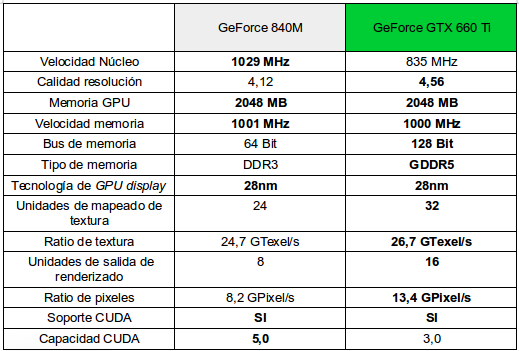
\includegraphics[width=1\linewidth]{../images/especificaciones}
	\caption[Especificaciones de las tarjetas 840M y GTX660]{Especificaciones de las tarjetas 840M y GTX660}
	\label{fig:especificaciones}
\end{figure}

\bigskip
Como nota hay que destacar el parámetro de \textit{capability} (capacidad), que será el que mayores restricciones o mejoras imponga en sus distintas versiones. Cuanto mayor sea esta, más funcionalidades podrá realizar y soportará más requisitos técnicos.

\bigskip
En la siguiente gráfica (Figura \ref{fig:grafico_benchmarks}) se verá la diferencia de ambas en benchmarks para medir \underline{procesamiento de gráficos} (Parallax, MRender, Gravity y Splatting):

\begin{figure}[h]
	\centering
	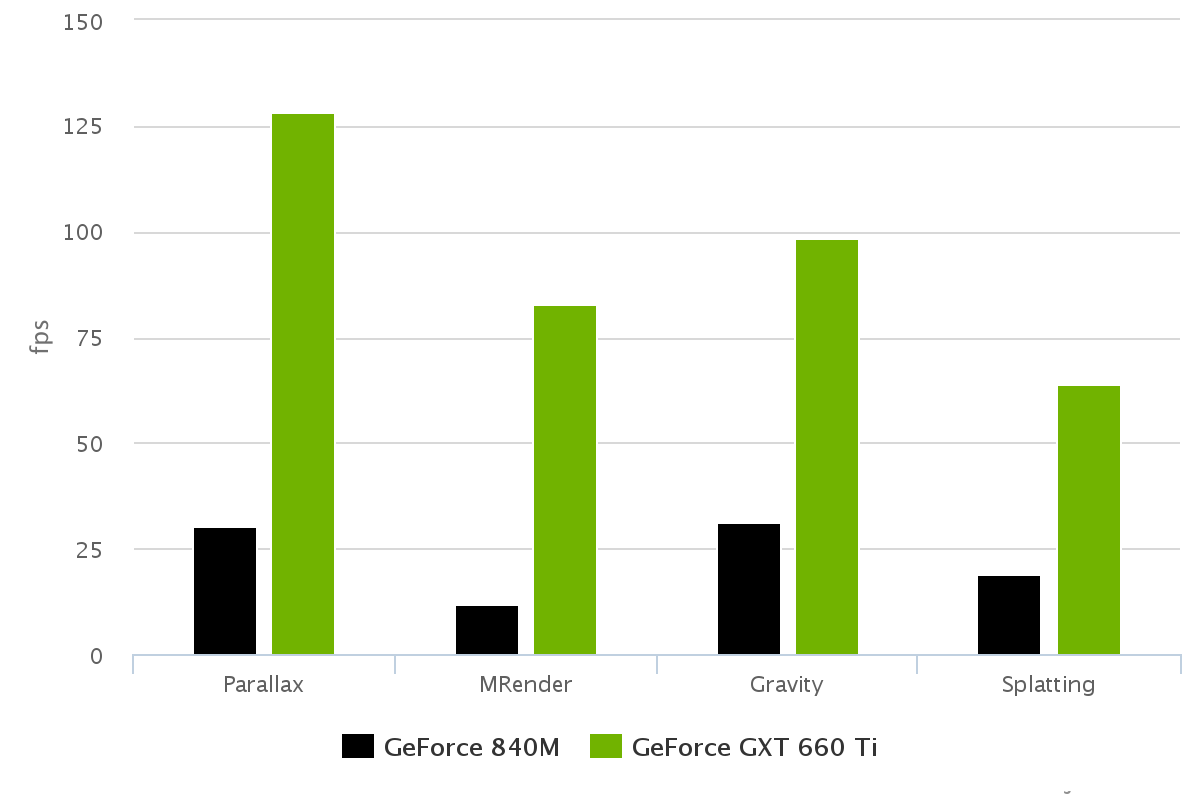
\includegraphics[width=0.6\linewidth]{../images/grafico_benchmarks}
	\caption[Comparativa de las tarjetas mediante bencharks de GPU]{Comparativa de las tarjetas mediante bencharks de GPU}
	\label{fig:grafico_benchmarks}
\end{figure}


\newpage %\bigskip
Pero en el ámbito de la computación mediante GPU con CUDA tendremos hay que fijarse en la capacidad de cada modelo de tarjeta, ya que una versión más actualizada puede lograr mejores resultados aunque tenga peores especificaciones \cite{capacidadescuda}.

\bigskip
Para ello se verán los tiempos que emplean ambas tarjetas (con distintas capacidades \cite{capacidades}) para varios números de generaciones:

\bigskip
\begin{figure}[h]
	\centering
	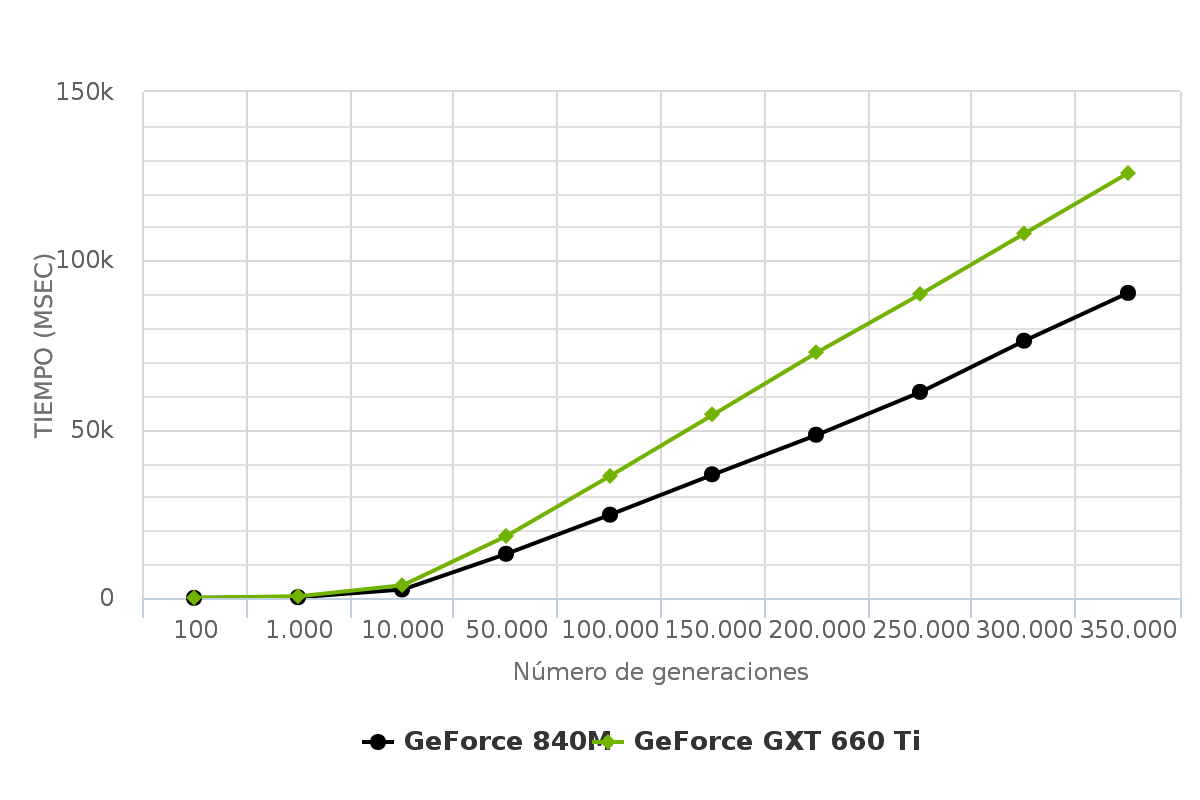
\includegraphics[width=0.9\linewidth]{../images/grafico_tiempos}
	\caption[Comparativa de tiempos entre tarjetas]{Comparativa de tiempos entre tarjetas}
	\label{fig:grafico_tiempos}
\end{figure}

\bigskip
Y se ve que la tarjeta con mejores prestaciones pero peor capacidad (GeForce GTX 660 Ti) tarda más en ejecutar los mismos procesamientos que hace la tarjeta con peores prestaciones pero mejor capacidad (GeForce 840M).

\bigskip
Como conclusión se llega a que a la hora de escoger el dispositivo a usar por el sistema para realizar los cómputos no sólo habrá que tener en cuenta los requisitos, si no que el factor de capacidad será decisivo para el rendimiento del cómputo y con ello del sistema.

También que ambas producen buenos resultados en el sistema, por lo que, se podría usar cualquiera en el sistema.

